\chapter{Lecture 1: Topics in String Theory}

These notes follow Leonard Susskind's first lecture in the supplementary track on cosmology and black holes. The lecture begins with a philosophical challenge to reductionism and then steadily sharpens that challenge into a sequence of mathematical examples: bosonization in \(1+1\) dimensions, electric--magnetic duality in quantum electrodynamics, the appearance of D-branes in string theory, strong-coupling transitions, emergent geometry, and finally the combinatorial landscape of string vacua. The aim here is to preserve the lecture's order, rhythm, and motivation while giving the mathematics a cleaner written form. Based on a lecture by Leonard Susskind; notes curated by LazyingArt LLC.

\section{Reductionism, Complexity, and the Question of Simplicity}

Susskind opens with a deliberately familiar philosophical slogan: big things are made of little things, and little things are made of littler things. He then adds the more ambitious version of the same idea, the one that really matters for fundamental physics: as one descends through deeper layers, the objects should become not only smaller but also simpler. His metaphor is that houses are made of bricks, and nobody mistakes a house for a brick. The brick is smaller, but it is also simpler.

The first move of the lecture is to confront that expectation with the actual state of particle physics. If reductionism were delivering increasing simplicity in that strong sense, one might expect present-day elementary particle physics to be close to economical. Instead, Susskind emphasizes that even before quantum gravity enters, the bookkeeping already looks messy. In the lecture these are rough counts, but the roughness is part of the point:
\begin{equation}
N_{\mathrm{species}} \sim 75,
\qquad
N_{\mathrm{independent}} \sim 10\text{--}20,
\qquad
N_{\mathrm{parameters}} \sim 20.
\end{equation}
Even this is not the end of the story. The Standard Model does not contain gravity, does not explain dark matter, does not supply the extra structure needed for inflation, and carries a severe fine-tuning problem. Once one adds the ``bells and whistles'' that are usually invoked to repair these omissions, the effective count swells rather than shrinks. In the lecture supersymmetry is the clean example, and the schematic message is simply
\begin{equation}
N_{\mathrm{parameters}}^{\mathrm{extended}} \sim 200.
\end{equation}

This quantitative complaint is not yet Susskind's main thesis. It is the prelude. The deeper claim, and the one that drives the rest of the lecture, is that modern quantum field theory and string theory do not obviously support a unique, coupling-independent distinction between the bricks and the houses. The next examples are chosen to show that the very meaning of ``elementary'' may depend on which variables are efficient.

\section{Bosonization: A First Breakdown of Fixed Fundamentality}

Susskind's first theoretical example comes from \(1+1\)-dimensional quantum field theory: one dimension of space, one of time. He announces at once that he is not going to derive the equivalence in detail; the point is not the formal proof but the conceptual lesson.

One starts with a field theory of fermions. The fermion field is denoted by \(\psi\). Two nearby fermions can form a bosonic composite, and the corresponding bosonic field is denoted by \(\phi\). At first sight the hierarchy seems straightforward: \(\psi\) is basic, while \(\phi\) is a composite or effective variable. In the lecture the boson is introduced exactly this way, as a field that creates bound pairs of fermions.

What was discovered, however, is that the same theory can be rewritten from the opposite starting point. One may begin with the bosonic field \(\phi\), and then the fermion no longer appears as a point-like constituent. Instead it appears as a kink of the bosonic field, an extended configuration in which \(\phi\) interpolates smoothly between two asymptotic values. The minimum mathematical content of the lecture is this asymptotic structure:
\begin{equation}
\phi(x\to -\infty)=\phi_-,
\qquad
\phi(x\to +\infty)=\phi_+.
\end{equation}
A convenient schematic representative is
\begin{equation}
\phi(x)\approx \frac{\phi_++\phi_-}{2}
+
\frac{\phi_+-\phi_-}{2}\tanh\!\left(\frac{x}{\ell}\right),
\end{equation}
where \(\ell\) is the width of the transition region. This is a standard reconstruction of the picture Susskind gives on the board; it is not meant to import a full sine-Gordon/Thirring derivation into a lecture that does not provide one.

The belt analogy in the lecture is precise enough to be worth keeping. A flat belt with no twist is a configuration with no kink. If one rotates one end by \(2\pi\), the belt returns to the same local orientation far away, but in between it must pass through an extended twisted region. That twisted region is the kink. In the bosonic description, the fermion is represented by precisely such an extended object.

The point becomes sharper once a coupling is introduced. Susskind calls it \(G\) in this example. The statement is not that the two descriptions are vaguely related, but that the efficiency of the two descriptions depends on the parameter regime:
\begin{align}
G \ll 1
&\Rightarrow
\ell \text{ small, the kink is tight, and the }\psi\text{-description is efficient},\\
G \gg 1
&\Rightarrow
\ell \text{ large, the kink spreads out, and the }\phi\text{-description is efficient}.
\end{align}
For small \(G\), the kink is tight and the fermion looks like the simple object. As \(G\) is increased, the kink broadens, the fermion becomes less point-like, and the bosonic variables become the more economical ones.

\paragraph{Schematic update rule.}
\begin{enumerate}
\item Begin with a fermionic theory described by \(\psi\).
\item Identify bosonic composites described by \(\phi\).
\item Rewrite the same theory entirely in terms of \(\phi\).
\item In the bosonic description, the fermion reappears as a kink of width \(\ell\).
\item For \(G\ll 1\), \(\ell\) is small and the fermionic description is simplest.
\item For larger \(G\), \(\ell\) grows and the bosonic description becomes simplest.
\end{enumerate}

This is the first explicit counterexample to the fixed ``houses and bricks'' picture. The lecture's punchline is not merely that composite objects exist, but that what counts as the elementary variable can change with the coupling.

\section{Electric Charge, Magnetic Monopoles, and Weak versus Strong Coupling}

Susskind next asks whether an analogous story appears in more familiar particle physics. The example is electric charge versus magnetic monopole. An ordinary charged particle, such as the electron, is an electric monopole in this language: a localized source of electric field. The magnetic monopole is introduced by the bar-magnet analogy. If one could somehow isolate the end of a bar magnet without the invisible connecting bar, the field lines would look exactly like those of an electric charge, but magnetic rather than electric.

The relevant control parameter is the fine-structure constant \(\alpha\). In the lecture Susskind treats it heuristically as the square of the electric charge:
\begin{equation}
\alpha \sim e^2.
\end{equation}
He also gives a rough operational interpretation: it measures how readily an electron radiates, and he summarizes that strength by saying that an accelerated electron radiates on the order of ``\(1/100\)'' photons in the relevant sense. In the lecture's own rough numerical language,
\begin{equation}
\alpha \approx 10^{-2}.
\end{equation}
This is not intended as a precision convention; it is a pedagogical way of encoding that electric charge is weak.

When \(\alpha\ll 1\), the electron is the simple object. Its electric field is weak, its vacuum polarization cloud is dilute, and it looks almost point-like. The magnetic monopole is then the opposite: its field is enormous, its surroundings are violently distorted, and it is broad, complicated, and heavy. Susskind summarizes the situation in precisely this weak--strong style:
\begin{align}
\alpha \ll 1
&\Rightarrow
\text{electron simple, monopole heavy and extended},\\
\alpha \gg 1
&\Rightarrow
\text{monopole simple, electron heavy and structured}.
\end{align}
The lecture does not derive a monopole mass formula. It does not need one. Its point is that as one increases \(\alpha\), the electron's field becomes stronger, the electron becomes surrounded by more structure, and the monopole shrinks and lightens. If \(\alpha\) were pushed far past unity, the convenient description would exchange: the monopole would be the simple object and the electron the complicated one.

That is the field-theory version of the earlier lesson from bosonization. The distinction between basic and composite is not absolute. It depends on the coupling.

\paragraph{A question about calculus.}
At this point a student asks whether calculus itself is an intrinsically reductionist tool. Susskind's answer is important because it briefly restates the whole philosophical point in different language. Calculus, he says, does not by itself tell us what the fundamental objects are; it only encodes smooth variation. The problem is that quantum fields do not behave like smooth classical fields on every scale. Rather, they fluctuate on all scales. There is no final clean layer at which the continuum simply reveals a unique set of smallest building blocks. This answer serves as a bridge: it closes the field-theory part of the argument and prepares the move to string theory.

\section{Strings, D-Branes, and the Return of Weak--Strong Duality}

The next transition in the lecture is deliberately naive. If string theory is supposed to be the theory of the fundamental building blocks, then surely the answer must be simple: the building blocks are strings. Susskind states that expectation openly, and then spends the next part of the lecture dismantling it.

\subsection{Why strings are not the whole story}

The first complication is the unavoidable presence of D-branes. A D\(p\)-brane is a \(p\)-dimensional object on which strings can end. The letter \(D\) comes from Dirichlet boundary conditions, but the name is far less important than the role: these objects are part of the theory and cannot be discarded. They are not optional ornaments.

The lecture begins with the simplest examples:
\begin{itemize}
\item a D0-brane, which is point-like,
\item a D1-brane, or D-string, which is string-like,
\item an F-string, the ordinary fundamental string.
\end{itemize}
A D0-brane is a heavy point-like site on which any number of F-strings can end. A D1-brane is a heavy cable-like object, much thicker and more massive per unit length than an F-string, but likewise a place where F-strings can end. At weak coupling the lecture does not present these objects as equally elementary alternatives. The D-branes are introduced as heavy, structured, composite-looking objects that the theory nevertheless forces upon us.

\paragraph{Notation.}
Susskind uses \(G\) and \(g\) somewhat loosely in different parts of the lecture. In these notes \(G\) is reserved for the bosonization example, while \(g\) denotes the string coupling.

The string coupling \(g\) is defined operationally, not axiomatically. It is the parameter that measures the probability that a fluctuating string splits and forms daughter strings. This is why Susskind compares it directly to the role of \(\alpha\) in QED. The lecture also pauses to identify tension with energy per unit length:
\begin{equation}
T=\frac{E}{L}=\frac{M}{L}.
\end{equation}

\subsection{F-strings and D-strings}

The weak--strong story then repeats itself in string language. At small coupling the F-string is light, thin, and close to the original intuitive image of the fundamental object. The D-string is thick, heavy, and full of F-string structure. As the coupling grows, the F-string splits more readily; the cloud of daughter strings proliferates around it, and it becomes heavier and more complicated. At the same time the D-string has increasing difficulty emitting the now-heavy F-strings, so its surrounding structure thins out and it becomes lighter and more line-like. The lecture's weak--strong map is therefore
\begin{align}
g \ll 1
&\Rightarrow
\text{F-string light and thin,\quad D-string heavy and structured},\\
g \sim 1
&\Rightarrow
\text{F-string and D-string look comparable},\\
g \gg 1
&\Rightarrow
\text{D-string light and thin,\quad F-string heavy and structured}.
\end{align}
Susskind remarks that around \(g\sim 1\) the two descriptions cease to be sharply distinct, and beyond that point they effectively exchange roles. This is the string-theoretic version of the electron--monopole interchange. The accepted name for this is S-duality.

The lecture pushes the point one step further. In the idealized theory the coupling is not merely a number to be dialed by hand; it behaves like a field. Schematically,
\begin{equation}
g = g(x).
\end{equation}
Different regions of space can therefore favor different dual descriptions. In one region F-strings are the light variables; in another region D-strings are. In between, nothing is especially simple. That is why, for Susskind, string theory does not restore the simple reductionist picture. It radicalizes the ambiguity.

\subsection{A question-driven return to quantum electrodynamics}

A student then asks whether the larger splitting probability simply means a more complicated structure ``upstream.'' Susskind answers by returning to quantum electrodynamics and drawing the electron's worldline again. This return matters: it shows that the string story is not an isolated curiosity but another instance of the same weak--strong pattern.

\begin{figure}[h]
\centering
\begin{tikzpicture}[scale=1.0]
\draw[->] (-1.2,0) -- (3.7,0) node[right] {space};
\draw[->] (0,-0.2) -- (0,4.3) node[above] {time};

\draw[line width=0.9pt] (0,0.2) -- (0,4.0);
\node[left] at (0,3.55) {\(e^{-}\)};

\draw[line width=0.8pt] (0,1.0) -- (0.18,1.08) -- (0.36,0.92) -- (0.54,1.10) -- (0.72,0.94) -- (0.90,1.12) -- (1.08,0.96) -- (1.26,1.14);
\draw[line width=0.8pt] (0,2.35) -- (-0.18,2.43) -- (-0.36,2.27) -- (-0.54,2.45) -- (-0.72,2.29) -- (-0.90,2.47);

\draw[line width=0.8pt] (1.26,1.14) -- (1.48,1.42);
\draw[line width=0.8pt] (1.26,1.14) -- (1.04,1.42);
\draw[line width=0.8pt] (1.48,1.42) -- (1.58,2.10);
\draw[line width=0.8pt] (1.04,1.42) -- (0.94,2.10);
\draw[line width=0.8pt] (0.94,2.10) -- (1.58,2.10);

\draw[line width=0.7pt] (1.58,1.78) -- (1.72,1.84) -- (1.86,1.72) -- (2.00,1.86);
\draw[line width=0.7pt] (0.94,1.78) -- (0.80,1.84) -- (0.66,1.72) -- (0.52,1.86);

\node at (2.35,1.95) {\(\gamma\)};
\node at (-1.15,2.75) {\(\gamma\)};
\end{tikzpicture}
\caption{Transcript-based redraw of Susskind's later QED recap. A point electron emits photons, photons create pairs, and the daughter charged lines radiate again, producing an endless hierarchy of finer structure.}
\end{figure}

The lecture's point is that even a point electron is accompanied by a hierarchy of processes:
\begin{enumerate}
\item an electron emits and absorbs photons,
\item a photon can create an electron--positron pair,
\item the daughter charged lines can themselves emit photons,
\item the hierarchy continues to smaller scales.
\end{enumerate}
For weak coupling this cloud is dilute, so the electron looks almost point-like in the laboratory. For stronger coupling it proliferates, and the electron becomes a structured object. The string story is then presented as a direct analogue of this.

The same later discussion also motivates Susskind's heuristic energy bookkeeping. He insists that the relevant energy is not merely the sum of free-particle contributions. One must also include interaction energy:
\begin{equation}
E_{\mathrm{tot}} = E_e + E_\gamma + E_{\mathrm{int}}.
\end{equation}
Here \(E_{\mathrm{int}}\) is the crucial term. It is what lets the mass of the dressed electron include the energy associated with its surrounding field and virtual structure. The lecture does not turn this into a formal renormalized self-energy derivation, and neither should these notes. The point is heuristic but essential: the object's mass already includes the interaction energy required to support the complicated cloud around it.

\begin{figure}[h]
\centering

\includegraphics[width=0.72\textwidth]{lecture_01_figure_02.png}

\vspace{1em}

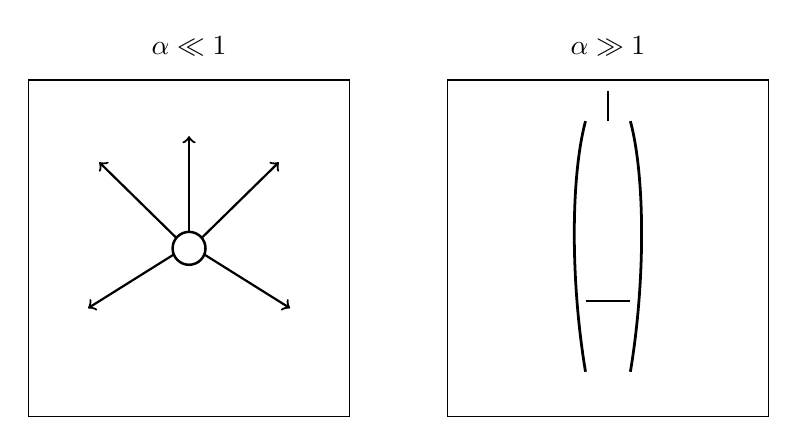
\begin{tikzpicture}[scale=0.95]
\draw (-5.3,-2.4) rectangle (-1.0,2.1);
\draw (0.3,-2.4) rectangle (4.6,2.1);

\node at (-3.15,2.55) {$\alpha \ll 1$};
\node at (2.45,2.55) {$\alpha \gg 1$};

\draw[line width=0.9pt] (-3.15,-0.15) circle (0.22);
\draw[->,line width=0.8pt] (-3.15,0.07) -- (-3.15,1.35);
\draw[->,line width=0.8pt] (-2.98,-0.01) -- (-1.95,1.00);
\draw[->,line width=0.8pt] (-3.32,-0.01) -- (-4.35,1.00);
\draw[->,line width=0.8pt] (-2.95,-0.23) -- (-1.80,-0.95);
\draw[->,line width=0.8pt] (-3.35,-0.23) -- (-4.50,-0.95);

\draw[line width=1.0pt] (2.15,-1.8) .. controls (1.95,-0.6) and (1.95,0.8) .. (2.15,1.55);
\draw[line width=1.0pt] (2.75,-1.8) .. controls (2.95,-0.6) and (2.95,0.8) .. (2.75,1.55);
\draw[line width=0.8pt] (2.15,-0.85) -- (2.75,-0.85);
\draw[line width=0.8pt] (2.45,1.55) -- (2.45,1.95);
\end{tikzpicture}
\caption{A later board recap of the weak--strong QED comparison. The screenshot is kept as evidence for the blackboard layout; the redraw records only the robust contrast between a compact weak-coupling object and an extended strong-coupling one.}
\end{figure}

The reason this figure belongs here, even though the weak--strong comparison was introduced earlier, is that in the lecture Susskind redraws the contrast at this later question-driven moment while discussing interaction energy and proliferating structure.

\section{Even-Brane Theories and the Emergent Extra Dimension}

Up to this point the lecture has been telling a strong story about exchange: fermion versus boson, electron versus monopole, F-string versus D-string. The next step is more surprising. Susskind switches to a different version of string theory, one with even-dimensional D-branes rather than odd-dimensional ones. The distinction matters because in this theory there is no D-string to exchange with the F-string. One has D0-branes, D2-branes, D4-branes, and so on.

The strong-coupling limit therefore cannot simply be a relabeling of one string as another. According to the lecture, something stranger happens: an extra spatial dimension becomes manifest. Susskind deliberately states this in the most dramatic form first --- ``a new dimension materializes'' --- and then immediately translates it into the more careful statement: a very small compact direction expands until it can no longer be ignored.

The bookkeeping is part of the point, so he pauses over it:
\begin{equation}
10\text{-dimensional string theory}=9\text{ space}+1\text{ time},
\qquad
11\text{-dimensional theory}=10\text{ space}+1\text{ time}.
\end{equation}
The lecture's claim is that the strong-coupling limit of the even-brane theory is effectively eleven-dimensional.

\subsection{The peanut-butter sandwich}

To picture the compact direction, Susskind uses the ``peanut-butter sandwich'' model: two infinitely thin pieces of bread, with real space between them. The special rule is that going out one side returns one to the other. In a conventional notation that the lecture describes pictorially rather than formally, one may write
\begin{equation}
y \sim y + 2\pi R.
\end{equation}
If \(R\) is very small, observers living in the sandwich effectively describe their world as lower-dimensional. The key strong-coupling update is then
\begin{equation}
g\uparrow
\qquad \Longrightarrow \qquad
R_{\mathrm{compact}}\uparrow.
\end{equation}
That is what Susskind means when he says that a new dimension of space appears: not that space is created from nothing, but that a previously tiny compact direction expands and becomes visible in the effective theory.

\begin{figure}[h]
\centering
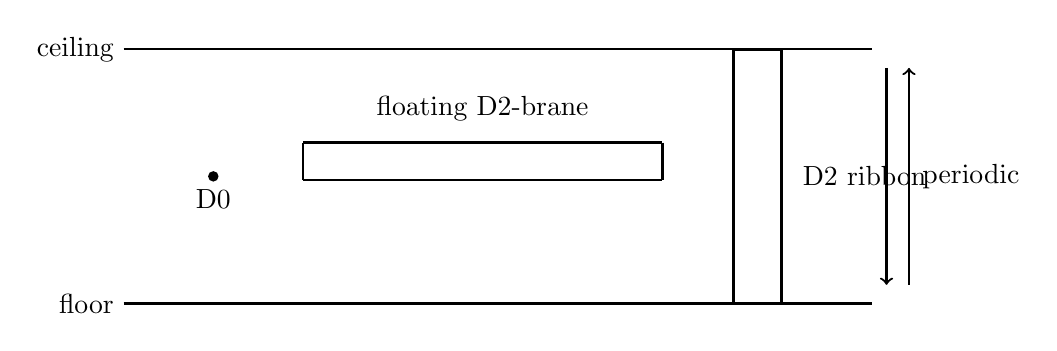
\begin{tikzpicture}[scale=0.95]
\draw[line width=0.9pt] (-5,1.7) -- (5,1.7);
\draw[line width=0.9pt] (-5,-1.7) -- (5,-1.7);

\node[left] at (-5,1.7) {ceiling};
\node[left] at (-5,-1.7) {floor};

\draw[->,line width=0.8pt] (5.2,1.45) -- (5.2,-1.45);
\draw[->,line width=0.8pt] (5.5,-1.45) -- (5.5,1.45);
\node[right] at (5.55,0) {periodic};

\draw[line width=1.0pt] (-2.6,0.45) -- (2.2,0.45);
\draw[line width=1.0pt] (-2.6,-0.05) -- (2.2,-0.05);
\draw[line width=1.0pt] (-2.6,0.45) -- (-2.6,-0.05);
\draw[line width=1.0pt] (2.2,0.45) -- (2.2,-0.05);
\node at (-0.2,0.9) {floating D2-brane};

\draw[line width=1.0pt] (3.15,-1.7) -- (3.8,-1.7);
\draw[line width=1.0pt] (3.15,1.7) -- (3.8,1.7);
\draw[line width=1.0pt] (3.15,-1.7) -- (3.15,1.7);
\draw[line width=1.0pt] (3.8,-1.7) -- (3.8,1.7);
\node[right] at (3.95,0) {D2 ribbon};

\fill (-3.8,0) circle (0.07);
\node[below] at (-3.8,-0.05) {D0};
\end{tikzpicture}
\caption{Transcript-based redraw of the sandwich compactification. The upper and lower boundaries are periodically identified; one D2-brane floats between them like a carpet, while another stretches from floor to ceiling and looks string-like when the compact direction is small.}
\end{figure}

\subsection{What becomes of the D0- and D2-branes?}

The lecture now asks what happens to the D0-branes and the strings. The answer is asymmetric. As \(g\) becomes large, the D0-branes get lighter and lighter; in the higher-dimensional interpretation they are simply gravitons carrying momentum in the newly manifest direction. Thus a heavy, complicated object in the weak-coupling picture becomes an ordinary light particle in the strong-coupling picture.

The D2-branes explain the fate of the strings. There are two configurations emphasized in the lecture:
\begin{enumerate}
\item a D2-brane floating between floor and ceiling like a carpet in the peanut butter;
\item a D2-brane stretched from floor to ceiling like a ribbon, extended along the visible direction.
\end{enumerate}
When the sandwich is thin, the ribbon looks effectively one-dimensional. It is the object that low-energy observers call a string. As the compact direction opens up, that same object becomes unmistakably membrane-like. Because it now contains more material in the vertical direction, it becomes heavy and unstring-like.

\paragraph{The logic of the transition.}
\begin{enumerate}
\item Start with a very thin compact direction, so the floor-to-ceiling ribbon behaves effectively like a string.
\item Increase \(g\), and the compact direction expands.
\item The D0-branes become light and are reinterpreted as gravitons in the higher-dimensional theory.
\item The string-like D2 ribbon becomes a visibly extended membrane and grows heavy.
\end{enumerate}
This is the lecture's hinge from duality to emergent geometry. Strong coupling does not merely exchange one object for another; it changes which geometry is the efficient one.

\section{D3-Branes, Wrapped Membranes, and a Geometrical Picture of Duality}

After the break Susskind explicitly describes the subject as an ``enormous web'' of interconnected theories and ideas. The next examples are not new isolated effects; they are bridges tying together the previous ones.

\subsection{A D3-brane worldvolume}

The first bridge uses a D3-brane. A D3-brane has three spatial dimensions, and an observer confined to it can easily mistake it for ordinary space. Strings can end on it, and from the worldvolume point of view the endpoint of a string looks like a particle.

\begin{figure}[h]
\centering
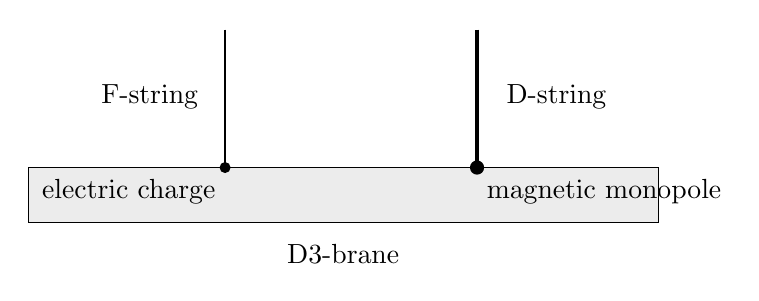
\begin{tikzpicture}[scale=1.0]
\draw[fill=gray!15] (-4,-0.35) rectangle (4,0.35);
\node at (0,-0.75) {D3-brane};

\draw[line width=0.9pt] (-1.5,2.1) -- (-1.5,0.35);
\fill (-1.5,0.35) circle (0.07);
\node[left] at (-1.72,1.25) {F-string};
\node[below left] at (-1.5,0.32) {electric charge};

\draw[line width=1.5pt] (1.7,2.1) -- (1.7,0.35);
\fill (1.7,0.35) circle (0.09);
\node[right] at (1.95,1.25) {D-string};
\node[below right] at (1.7,0.32) {magnetic monopole};
\end{tikzpicture}
\caption{Transcript-based redraw of the D3-brane worldvolume interpretation. An F-string endpoint appears as an electrically charged particle; a D-string endpoint appears as a magnetic monopole.}
\end{figure}

This is one of the lecture's most satisfying identifications. An F-string ending on the D3-brane appears to the worldvolume observer as an electric charge. A D-string ending on the same brane appears as a magnetic monopole. In other words, the duality between F-strings and D-strings becomes, on the D3-brane worldvolume, the electric--magnetic duality of ordinary field theory. What was earlier an analogy is now an explicit dictionary.

\subsection{Two compact directions and asymmetric wrapping}

Susskind then returns to the higher-dimensional geometry and compactifies not one but two small directions. Since one cannot draw eleven dimensions on a blackboard, he compresses the picture to one visible large direction and two compact ones. He insists on drawing the compactification asymmetrically, because one direction must be shorter than the other if the effective strings are to have different tensions.

\begin{figure}[h]
\centering

\includegraphics[width=0.78\textwidth]{lecture_01_figure_03.png}

\vspace{1em}

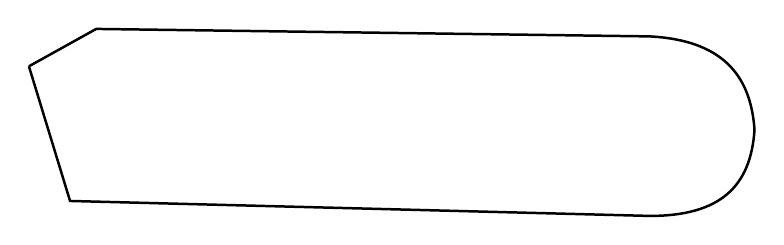
\begin{tikzpicture}[scale=0.95]
\draw[line width=0.9pt]
(-5,0.85) -- (-4.1,1.35) -- (3.3,1.25)
.. controls (4.25,1.20) and (4.65,0.75) .. (4.7,0.00)
.. controls (4.65,-0.75) and (4.25,-1.15) .. (3.3,-1.15)
-- (-4.45,-0.95) -- (-5,0.85);
\end{tikzpicture}
\caption{The asymmetric profile introduced when Susskind says he will draw the picture asymmetrically. The screenshot is kept because the argument here is strongly visual; the redraw regularizes only the large-scale asymmetry.}
\end{figure}

The clean mathematical content is then as follows. A membrane may wrap one compact direction and produce one effective string, or it may wrap the other compact direction and produce another. Since the compact directions do not have the same size, the two effective strings do not have the same tension. If \(R_1\) and \(R_2\) denote the two compact scales, then the lecture's later interpretation is that the weak--strong parameter is encoded geometrically as the aspect ratio
\begin{equation}
\alpha \sim \frac{R_1}{R_2}.
\end{equation}
Here the notation shifts: \(\alpha\) is no longer the QED fine-structure constant. It now denotes a geometric ratio. The lecture says this explicitly in response to a student question, and the shift should be flagged because the same symbol is being reused for a different purpose.

\begin{remark}
In the geometric part of the lecture, \(\alpha\) is being reinterpreted as an aspect-ratio parameter. The symbol is the same as before, but the meaning is different.
\end{remark}

A clean transcript-backed reconstruction of the wrapped-membrane picture is:

\begin{figure}[h]
\centering
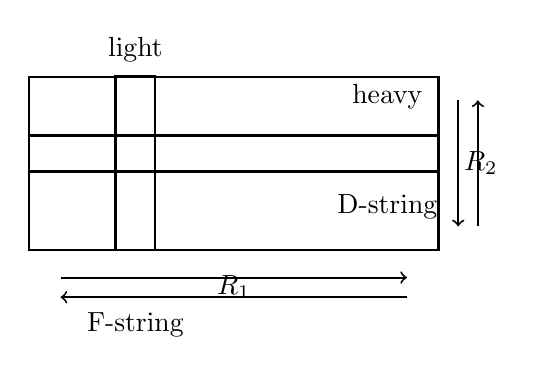
\begin{tikzpicture}[scale=1.0]
\draw[line width=0.9pt] (0,0) rectangle (5.2,2.2);
\node[below] at (2.6,-0.2) {\(R_1\)};
\node[right] at (5.4,1.1) {\(R_2\)};

\draw[->,line width=0.7pt] (5.45,1.9) -- (5.45,0.3);
\draw[->,line width=0.7pt] (5.7,0.3) -- (5.7,1.9);
\draw[->,line width=0.7pt] (0.4,-0.35) -- (4.8,-0.35);
\draw[->,line width=0.7pt] (4.8,-0.6) -- (0.4,-0.6);

\draw[line width=1.0pt] (1.1,0) -- (1.6,0) -- (1.6,2.2) -- (1.1,2.2) -- cycle;
\node at (1.35,2.55) {light};

\draw[line width=1.0pt] (0,1.45) -- (5.2,1.45);
\draw[line width=1.0pt] (0,1.00) -- (5.2,1.00);
\node at (4.55,1.95) {heavy};

\node at (1.35,-0.95) {F-string};
\node at (4.55,0.55) {D-string};
\end{tikzpicture}
\caption{Clean reconstruction of the two-cycle picture. Two wrapped membrane configurations both look string-like from the non-compact directions, but unequal compact scales make one effective string lighter than the other.}
\end{figure}

This is the geometric version of the earlier duality story. Squeezing one direction while stretching the other makes one wrapped object heavier and the other lighter, so the roles of F-string and D-string can interchange.

\begin{figure}[h]
\centering

\includegraphics[width=0.78\textwidth]{lecture_01_figure_04.png}

\vspace{1em}

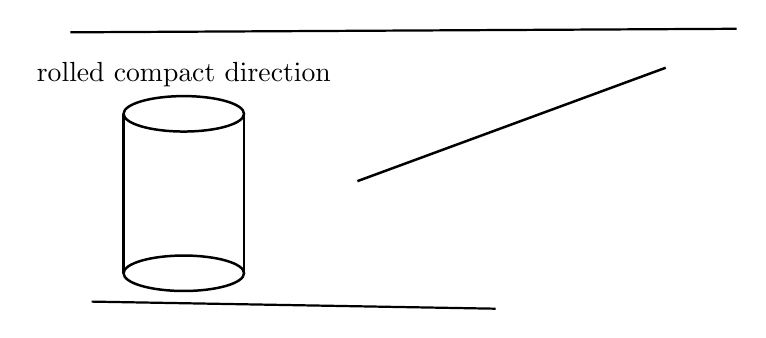
\begin{tikzpicture}[scale=0.9]
\draw[line width=0.9pt] (-3.6,0.9) ellipse (0.85 and 0.25);
\draw[line width=0.9pt] (-4.45,0.9) -- (-4.45,-1.35);
\draw[line width=0.9pt] (-2.75,0.9) -- (-2.75,-1.35);
\draw[line width=0.9pt] (-3.6,-1.35) ellipse (0.85 and 0.25);

\draw[line width=0.8pt] (-5.2,2.05) -- (4.2,2.10);
\draw[line width=0.8pt] (-4.9,-1.75) -- (0.8,-1.85);
\draw[line width=0.9pt] (-1.15,-0.05) -- (3.2,1.55);

\node at (-3.6,1.45) {rolled compact direction};
\end{tikzpicture}
\caption{The lecture's ``geometrical picture.'' The screenshot is kept as evidence for the actual board state; the redraw records only the cylinder-like compact direction, the long upper contour, and the slanted continuation that survive the occlusion.}
\end{figure}

At this point a student asks why the picture is not a helix rather than a circle. Susskind's answer is revealing. The geometry should be thought of as a compact direction cut open and drawn flat, so that exiting one side means re-entering at the identified side. The lecture emphasizes that this is a geometrical picture, useful but not exhaustive. It organizes the duality, but it does not by itself explain every microscopic feature of how a D-brane, under sufficiently hard probing, can look like a collection of F-strings.

\section{Idealization, Specially Symmetric Points, and the Landscape}

The last movement of the lecture steps back from the elegant duality examples and asks what they do, and do not, tell us about the real world.

First, Susskind warns that the precisely controlled dualities are features of highly idealized supersymmetric theories. His analogy is to circular orbits in Newtonian mechanics: one studies them first because they are symmetric and mathematically tractable, not because actual planetary motion is exhausted by perfect circles. In exactly the same way, supersymmetric string theories are easier to analyze because they are more symmetric than nature appears to be.

Within those idealized theories there are specially symmetric points. In the geometric picture these are the equal-aspect configurations,
\begin{equation}
R_1 = R_2,
\end{equation}
at which the two wrapped descriptions coincide. The corresponding field-theory statement is that the electric and magnetic descriptions are equally simple:
\begin{equation}
m_{\mathrm{monopole}} = m_e.
\end{equation}
Susskind immediately adds the physical caveat that our world does not seem to live at such a point; it is lopsided rather than symmetric.

\begin{figure}[h]
\centering

\includegraphics[width=0.78\textwidth]{lecture_01_figure_06.png}

\vspace{1em}

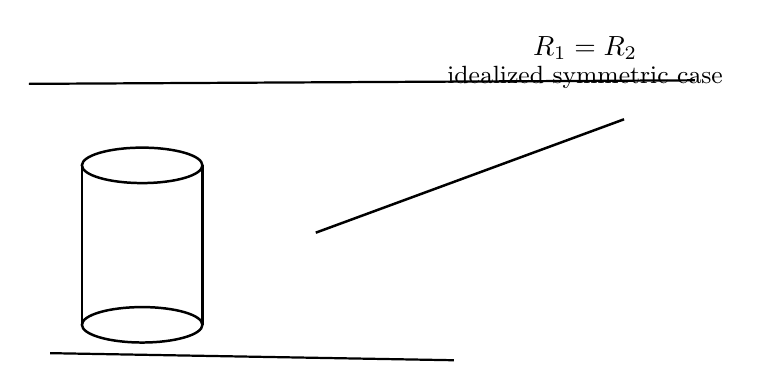
\begin{tikzpicture}[scale=0.9]
\draw[line width=0.9pt] (-3.6,0.9) ellipse (0.85 and 0.25);
\draw[line width=0.9pt] (-4.45,0.9) -- (-4.45,-1.35);
\draw[line width=0.9pt] (-2.75,0.9) -- (-2.75,-1.35);
\draw[line width=0.9pt] (-3.6,-1.35) ellipse (0.85 and 0.25);

\draw[line width=0.8pt] (-5.2,2.05) -- (4.2,2.10);
\draw[line width=0.8pt] (-4.9,-1.75) -- (0.8,-1.85);
\draw[line width=0.9pt] (-1.15,-0.05) -- (3.2,1.55);

\node at (2.65,2.55) {$R_1=R_2$};
\node at (2.65,2.15) {\small idealized symmetric case};
\end{tikzpicture}
\caption{Later board frame retained during the discussion of specially symmetric points. The equal-aspect annotation is transcript-backed interpretation, not a direct transcription of visible chalk.}
\end{figure}

This leads naturally into the lecture's final large-scale moral. The examples one can describe cleanly are special precisely because they are special. The generic construction in a vast configuration space need not be elegant. Susskind illustrates this first with coding theory and then with DNA: mathematically structured examples are easy to analyze, but the space of possibilities is overwhelmingly larger than the space of neat examples. The same combinatorial point then becomes the ``landscape'' argument of string theory.

Suppose a compact space has roughly \(500\) cycles, and each cycle admits on the order of \(10\) different choices of wrapped branes, fluxes, or related structures. Then the number of resulting constructions grows schematically like
\begin{equation}
N_{\mathrm{vacua}} \sim 10^{500}.
\end{equation}
The lecture's counting logic is elementary:
\begin{equation}
10 \times 10 \times \cdots \times 10 = 10^{500}
\end{equation}
with \(500\) factors. The DNA analogy makes the same point in a more familiar register:
\begin{equation}
N_{\mathrm{DNA}}(500)=4^{500}.
\end{equation}
The exact exponents are not the point. The point is that simple local rules can generate a staggeringly large space of globally different constructions.

This gives Susskind's final inversion of the opening reductionist expectation. The complication of particle physics may not mean that the microscopic rules themselves are elaborate. It may instead mean that the vacuum we inhabit is one complicated member of an enormous family built from relatively simple ingredients.

The last coda of the lecture turns briefly toward cosmology. A compact spatial direction that is sufficiently large is observationally hard to distinguish from an infinite one. Flatness, by itself, only gives lower bounds on size; it does not prove non-compactness. At the same time, Susskind stresses that the smoothly varying couplings of the idealized examples are not compatible with our world. If couplings vary at all in nature, the variations must be step-like rather than smooth, a point he postpones to later cosmological discussions.

\section{Summary}

The lecture begins with the philosophical hope that deeper layers of physics should be simpler and ends by showing how fragile that hope has become. In \(1+1\)-dimensional bosonization, the same theory can be organized either around fermions or around bosons, with the fermion reappearing as a kink. In quantum electrodynamics, weak and strong coupling exchange the descriptive roles of electron and magnetic monopole. In string theory, F-strings and D-strings repeat the same pattern, and in the even-brane theory strong coupling goes further still: a compact direction expands, D0-branes become gravitons, and the effective strings are reinterpreted as wrapped membranes in a higher-dimensional geometry. The final lesson is that modern quantum field theory and string theory do not furnish a unique once-and-for-all answer to the question ``which are the bricks and which are the houses?'' They furnish a web of descriptions, each efficient in its own regime, together with a huge landscape of possible constructions whose generic output is complexity rather than simplicity.